% Section
\section{Evaluation}
\label{sec:experiments}

The experiments presented hereafter evaluate the performance of our balancing methods when compared to an existing and effective task clustering strategy named Horizontal Clustering (HC)~\cite{Singh:2008:WTC:1341811.1341822}, which is widely used by workflow management systems such as Pegasus~\cite{Deelman2004}. We also compare our methods with two heuristics described in literature: DFJS~\cite{Muthuvelu:2005:DJG:1082290.1082297}, and AFJS~\cite{Liu2009}. DFJS groups bags of tasks based on the task durations up to the resource capacity. AFJS is an extended version of DFJS that is an adaptive fine-grained job scheduling algorithm to group fine-grained tasks according to processing capacity of the current available resources and bandwidth between these resources.

% Workflow applications
\subsection{Scientific workflow applications}
\label{sec:applications}

Five real scientific workflow applications are used in the experiments: LIGO Inspiral analysis~\cite{LIGO}, Montage~\cite{Berriman2004}, CyberShake~\cite{Graves2010}, Epigenomics~\cite{Epigenome}, and SIPHT~\cite{SIPHT}. In this subsection, we describe each workflow application and present their main characteristics and structures.

\paragraph{\textbf{LIGO}}
Laser Interferometer Gravitational Wave Observatory (LIGO)~\cite{LIGO} workflows are used to search for gravitational wave signatures in data collected by large-scale interferometers. The observatories' mission is to detect and measure gravitational waves predicted by general relativity (Einstein's theory of gravity), in which gravity is described as due to the curvature of the fabric of time and space. The LIGO Inspiral workflow is a data-intensive workflow. Figure~\ref{fig:evaluation_shape_ligo} shows a simplified version of this workflow. The LIGO Inspiral workflow is separated into multiple groups of interconnected tasks, which we call branches in the rest of our paper. However, each branch may have a different number of pipelines as shown in Figure~\ref{fig:evaluation_shape_ligo}. 

\begin{figure}[!htb]
	\centering
	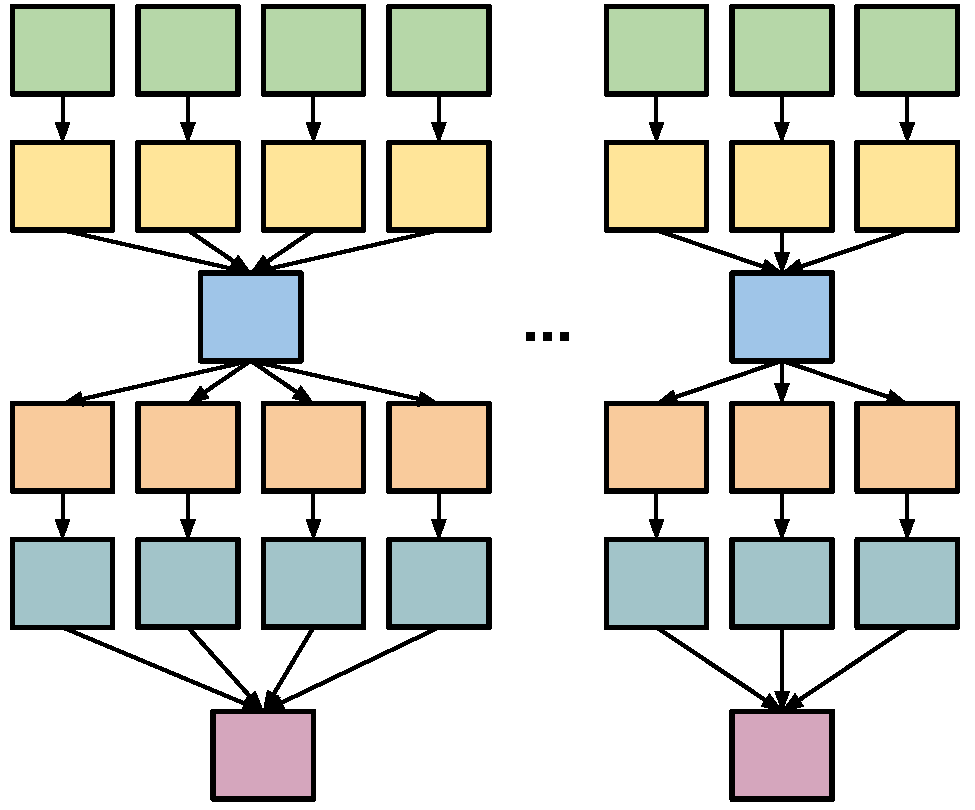
\includegraphics[width=0.5\linewidth]{figure14.pdf} \\
	\caption{A simplified visualization of the LIGO Inspiral workflow.}
	\label{fig:evaluation_shape_ligo}
\end{figure}

\paragraph{\textbf{Montage}}
Montage~\cite{Berriman2004} is an astronomy application that is used to construct large image mosaics of the sky. Input images are reprojected onto a sphere and overlap is calculated for each input image. The application re-projects input images to the correct orientation while keeping background emission level constant in all images. The images are added by rectifying them to a common flux scale and background level. Finally the reprojected images are co-added into a final mosaic. The resulting mosaic image can provide a much deeper and detailed understanding of the portion of the sky in question. Figure~\ref{fig:evaluation_shape_montage} illustrates a small Montage workflow. The size of the workflow depends on the number of images used in constructing the desired mosaic of the sky. The structure of the workflow changes to accommodate increases in the number of inputs, which corresponds to an increase in the number of computational tasks.

\begin{figure}[htb]
	\centering
	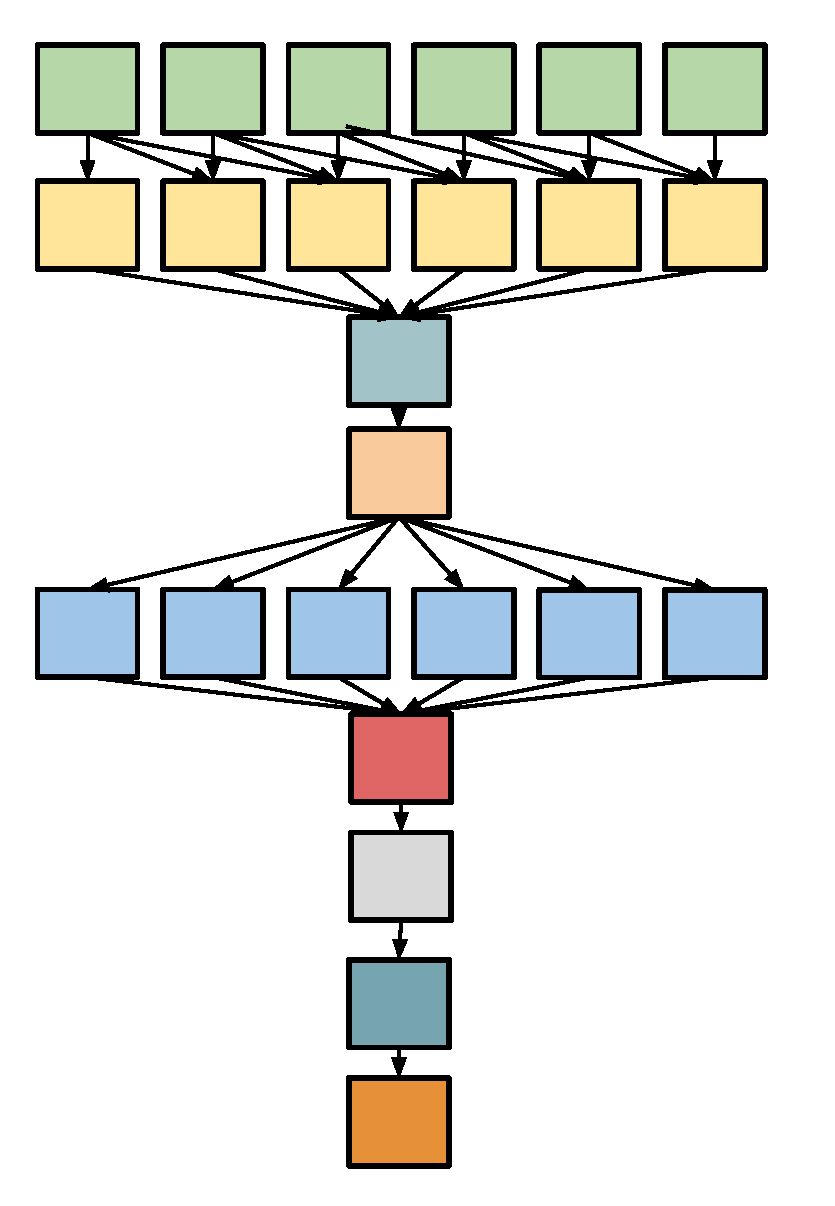
\includegraphics[width=0.4\linewidth]{figure15.pdf} \\
	\caption{A simplified visualization of the Montage workflow.}
	\label{fig:evaluation_shape_montage}
\end{figure}

\paragraph{\textbf{Cybershake}}
CyberShake~\cite{Graves2010} is a seismology application that calculates Probabilistic Seismic Hazard curves for geographic sites in the Southern California region. It identifies all ruptures within 200km of the site of interest and converts rupture definition into multiple rupture variations with differing hypocenter locations and slip distributions. It then calculates synthetic seismograms for each rupture variance, and peak intensity measures are then extracted from these synthetics and combined with the original rupture probabilities to produce probabilistic seismic hazard curves for the site. Figure~\ref{fig:evaluation_shape_cybershake} shows an illustration of the Cybershake workflow.

\begin{figure}[htb]
	\centering
	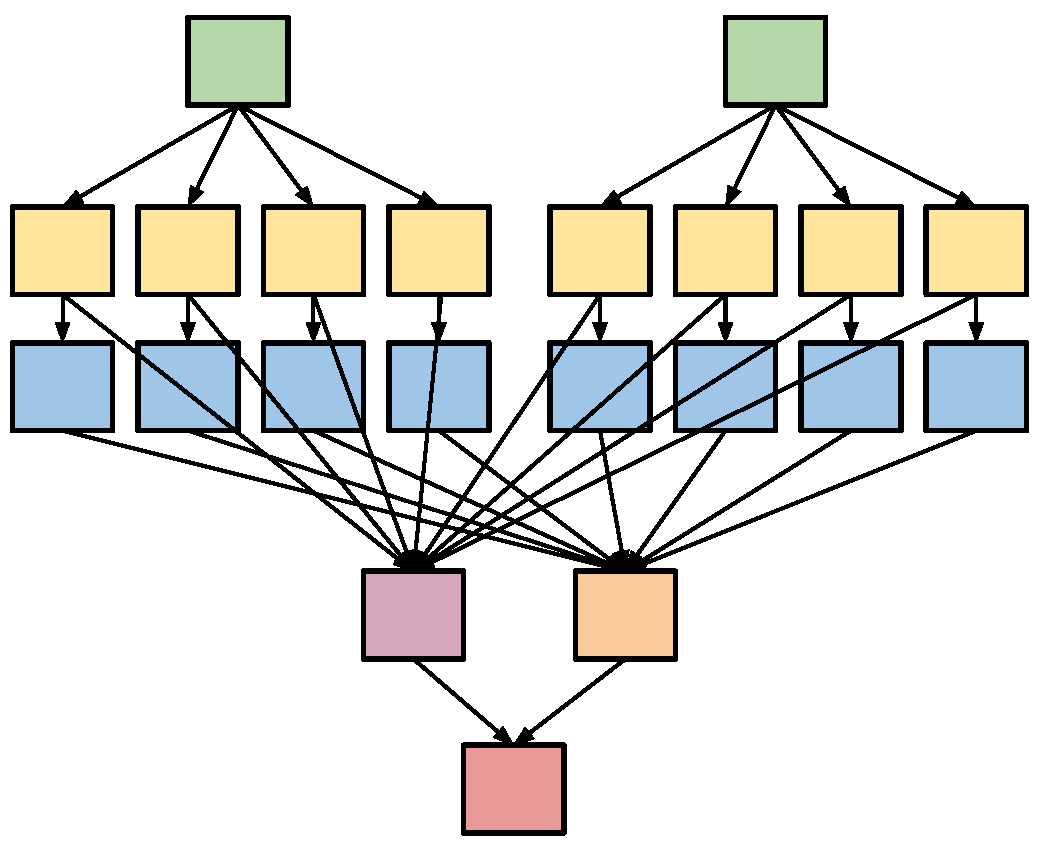
\includegraphics[width=0.55\linewidth]{figure16.pdf} \\
	\caption{A simplified visualization of the CyberShake workflow.}
	\label{fig:evaluation_shape_cybershake}
\end{figure}

\paragraph{\textbf{Epigenomics}}
The Epigenomics workflow~\cite{Epigenome} is a data-parallel workflow. Initial data are acquired from the Illumina-Solexa Genetic Analyzer in the form of DNA sequence lanes. Each Solexa machine can generate multiple lanes of DNA sequences. These data are converted into a format that can be used by sequence mapping software. The mapping software can do one of two major tasks. It either maps short DNA reads from the sequence data onto a reference genome, or it takes all the short reads, treats them as small pieces in a puzzle and then tries to assemble an entire genome. In our experiments, the workflow maps DNA sequences to the correct locations in a reference Genome. This generates a map that displays the sequence density showing how many times a certain sequence expresses itself on a particular location on the reference genome. Epigenomics is a CPU-intensive application and its simplified structure is shown in Figure~\ref{fig:evaluation_shape_genome}. Different to the LIGO Inspiral workflow, each branch in Epigenomics has exactly the same number of pipelines, which makes it more symmetric. 

\begin{figure}[htb]
	\centering
	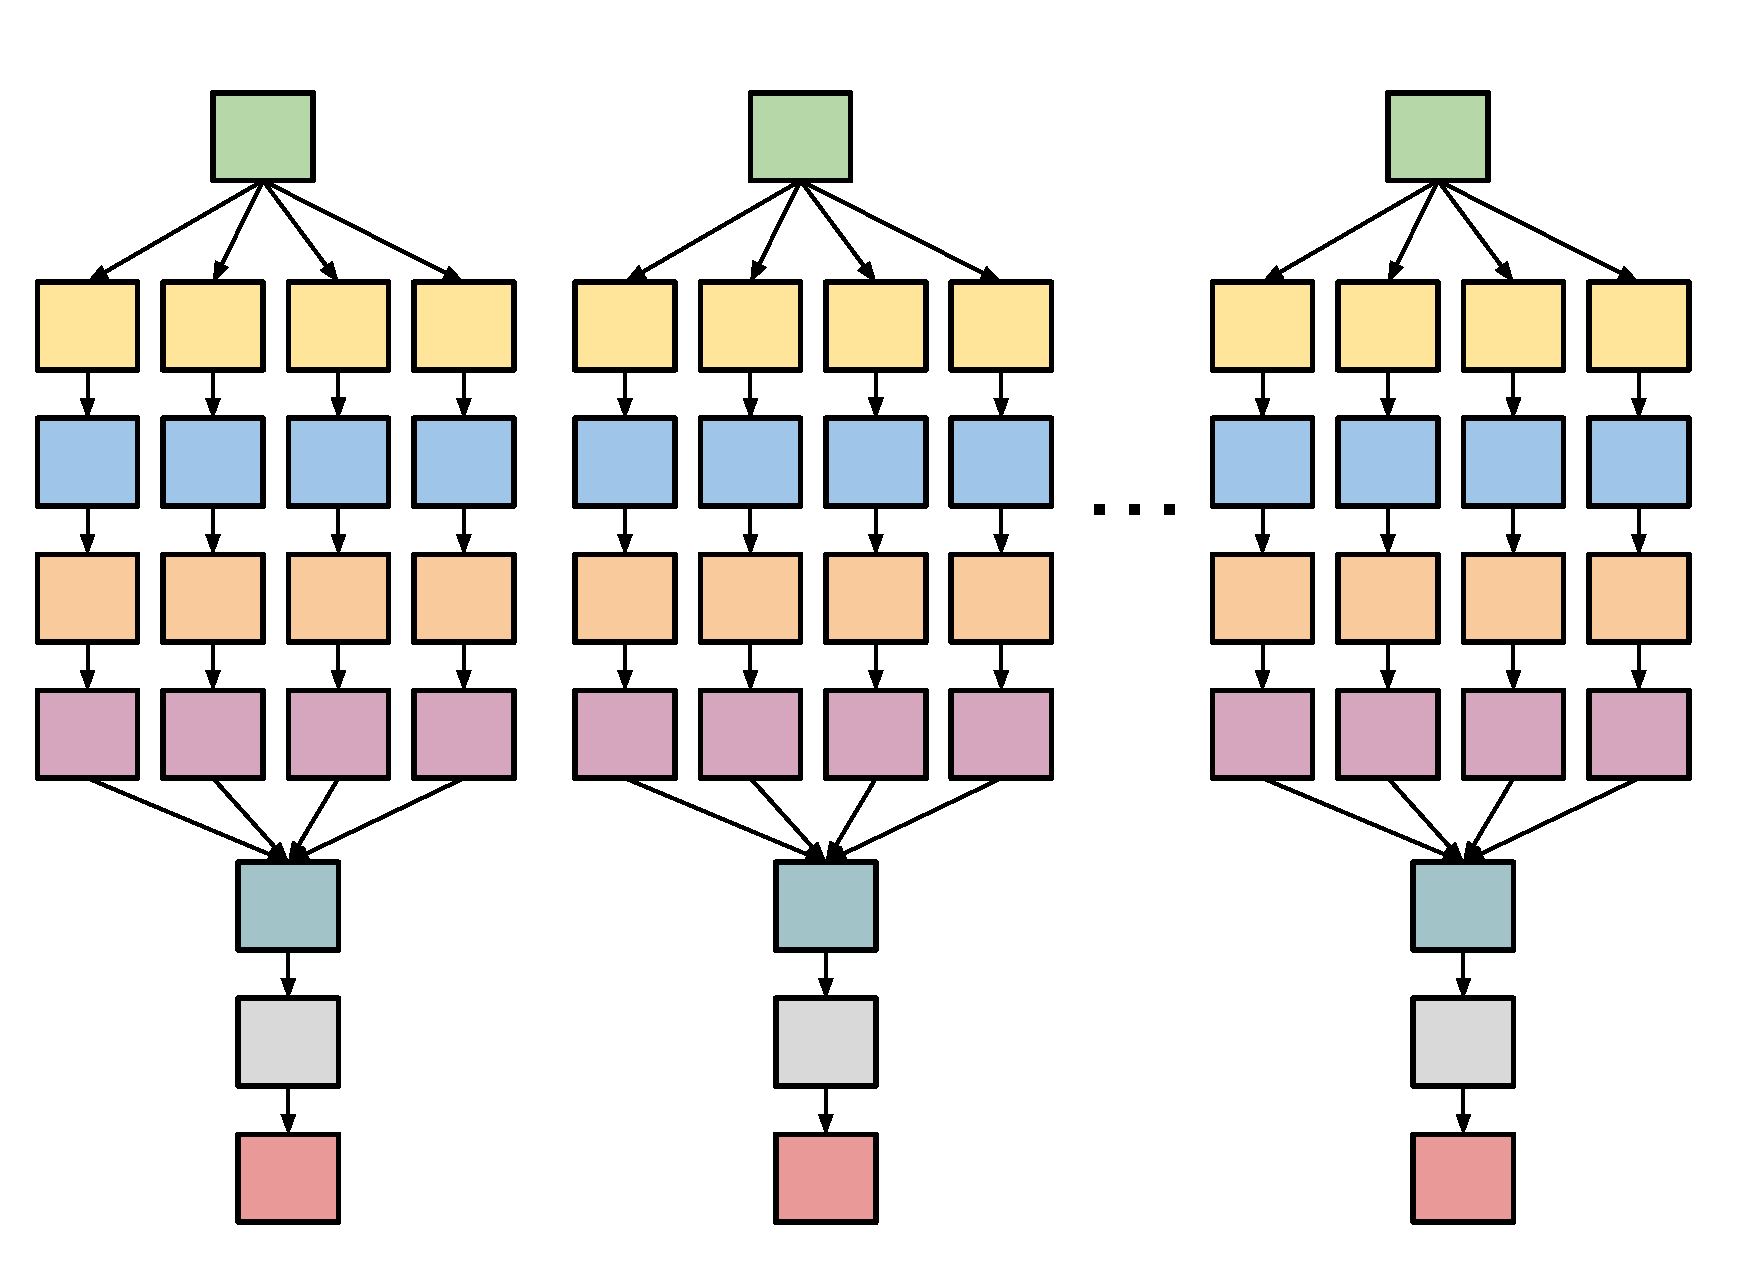
\includegraphics[width=.85\linewidth]{figure17.pdf} \\
	\caption{A simplified visualization of the Epigenomics workflow with multiple branches.}
	\label{fig:evaluation_shape_genome}
\end{figure}

\paragraph{\textbf{SIPHT}}
The SIPHT workflow~\cite{SIPHT} conducts a wide search for small untranslated RNAs (sRNAs) that regulates several processes such as secretion or virulence in bacteria. The kingdom-wide prediction and annotation of sRNA encoding genes involves a variety of individual programs that are executed in the proper order using Pegasus~\cite{Deelman2004}. These involve the prediction of $\rho$-independent transcriptional terminators, BLAST (Basic Local Alignment Search Tools) comparisons of the inter genetic regions of different replicons and the annotations of any sRNAs that are found. A simplified structure of the SIPHT workflow is shown in Figure~\ref{fig:evaluation_shape_sipht}. 

\begin{figure}[htb]
	\centering
	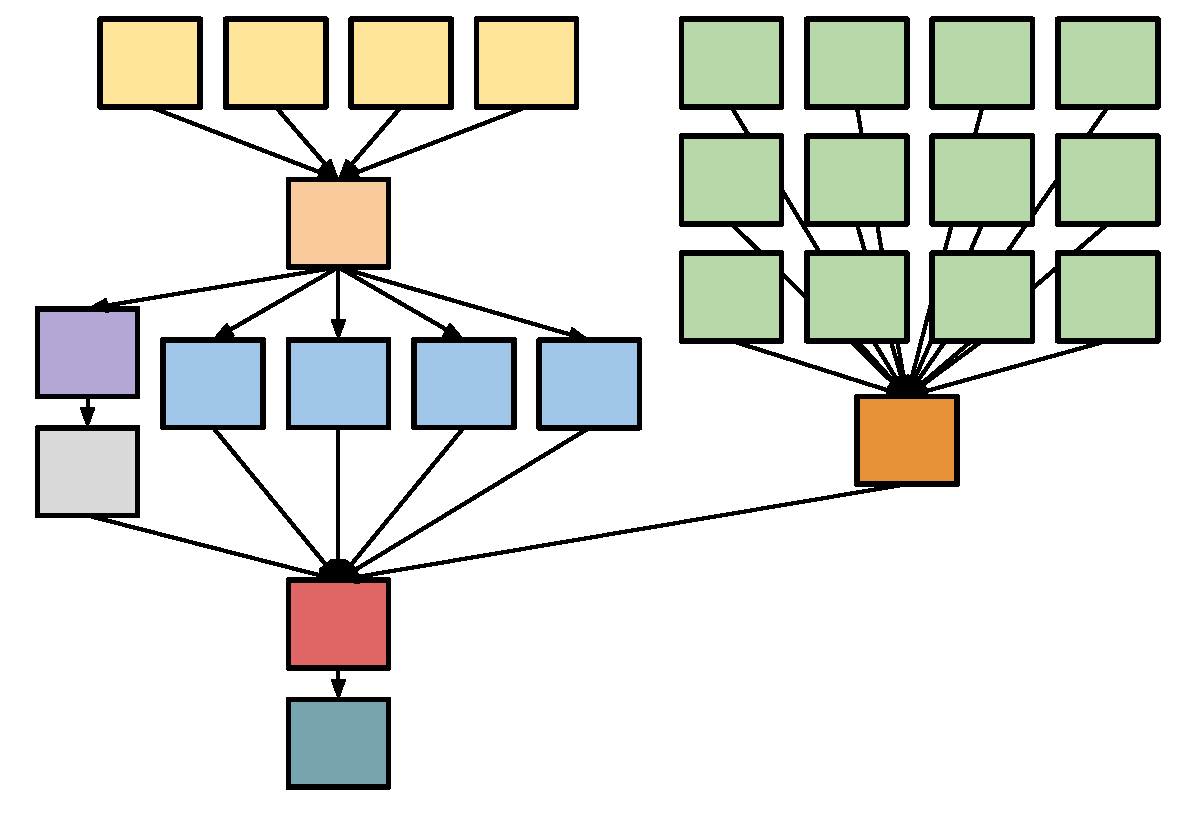
\includegraphics[width=0.6\linewidth]{figure18.pdf} \\
	\caption{A simplified visualization of the SIPHT workflow.}
	\label{fig:evaluation_shape_sipht}
\end{figure}


\begin{table}[!htb]
	\setlength{\tabcolsep}{11pt}
	\centering
	\small
	\begin{tabular}{lrrrr}
		\hline
		 & \multicolumn{1}{c}{Number} & \multicolumn{1}{c}{Average} &  \multicolumn{1}{c}{Average} \\
		Workflow	& of Tasks	 & Data Size & Task Runtime \\
		\hline
		LIGO 		&800		& 5 MB	& 228s\\
		Montage 		&300		&3 MB	&11s\\
		CyberShake 	&700		&148 MB 	& 23s\\
		Epigenomics 	&165 	& 355 MB	& 2952s\\
		SIPHT		&1000	& 360 KB 	& 180s\\
		\hline
	\end{tabular}
	\caption{Summary of the scientific workflows characteristics.}
	\label{tab:evaluation_workflows}
\end{table} 

Table~\ref{tab:evaluation_workflows} shows the summary of the main \textbf{workflows characteristics}: number of tasks, average data size, and average task runtimes for the five workflows. 


% Task clustering techniques
\subsection{Task clustering techniques}

In the experiments, we compare the performance of our balancing methods to the Horizontal Clustering (HC)~\cite{Singh:2008:WTC:1341811.1341822} technique, and with two methods well known from the literature, DFJS~\cite{Muthuvelu:2005:DJG:1082290.1082297} and AFJS~\cite{Liu2009}. In this subsection, we briefly describe each of these algorithms.


\paragraph{\textbf{HC}}
Horizontal Clustering (HC) merges multiple tasks that are at the same horizontal level of the workflow. The clustering granularity (number of tasks within a cluster) of a clustered job is controlled by the user, who defines either the number of tasks per clustered job (\emph{clusters.size}), or the number of clustered jobs per horizontal level of the workflow (\emph{clusters.num}). This algorithm has been implemented and used in Pegasus~\cite{Singh:2008:WTC:1341811.1341822}. For simplicity, we define \emph{clusters.num} as the number of available resources. In our prior work~\cite{6683907}, we have compared the runtime performance with different clustering granularity. The pseudocode of the HC technique is shown in Algorithm~\ref{alg:evaluation_hc}. 


\begin{algorithm}[!htb]
	\footnotesize
	\caption{Horizontal Clustering algorithm.}
	\label{alg:evaluation_hc}
	\begin{algorithmic}[1]
		\Require $W$: workflow; $C$: max number of tasks per job defined by \emph{clusters.size} or \emph{clusters.num}
		\Procedure{Clustering}{$W,C$}
			\For{$level < depth(W)$}
				\State $TL\gets $\ \Call{GetTasksAtLevel}{$W,level$} \Comment{Partition $W$ based on depth}
				\State $CL\gets$  \ \Call{Merge}{$TL,C$} \Comment{Returns a list of clustered jobs}
				\State $W \gets W - TL + CL$  \Comment{Merge dependencies as well} 
			\EndFor
		\EndProcedure
		\Procedure{Merge}{$TL, C$}
			\State $J\gets$ \{\}\Comment{An empty job}
			\State $CL\gets$\{\}\Comment{An empty list of clustered jobs}
			\While{$TL$ is not empty}
				\State $J$.add ($TL$.pop($C$) \Comment{Pops $C$ tasks that are not merged }
				\State  $CL$.add( $J$)
			\EndWhile
			\State \textbf{return} $CL$
		\EndProcedure
	\end{algorithmic}
\end{algorithm}

\paragraph{\textbf{DFJS}}
The dynamic fine-grained job scheduler (DFJS) was proposed by Muthuvelu et al.~\cite{Muthuvelu:2005:DJG:1082290.1082297}. The algorithm groups bags of tasks based on their granularity size---defined as the processing time of the task on the resource. Resources are ordered by their decreasing values of capacity (in MIPS), and tasks are grouped up to the resource capacity. This process continues until all tasks are grouped and assigned to resources. Algorithm~\ref{alg:evaluation_dfjs} shows the pseudocode of the heuristic. 
 
\begin{algorithm}[!htb]
	\caption{ DFJS algorithm.}
	\footnotesize
	\label{alg:evaluation_dfjs}
	\begin{algorithmic}[1]
		\Require $W$: workflow; $max.runtime$: max runtime of clustered jobs 
		\Procedure{Clustering}{$W,max.runtime$}
			\For{$level < $the depth of $W$}
				\State $TL\gets $\ \Call{GetTasksAtLevel}{$W,level$} \Comment{Partition $W$ based on depth}
				\State $CL\gets$  \ \Call{Merge}{$TL,max.runtime$} \Comment{Returns a list of clustered jobs}
				\State $W \gets W - TL + CL$  \Comment{Merge dependencies as well} 
			\EndFor
		\EndProcedure
		\Procedure{Merge}{$TL, max.runtime$}
			\State $J\gets$ \{\}\Comment{An empty job}
			\State $CL\gets$\{\}\Comment{An empty list of clustered jobs}
			\While{$TL$ is not empty}
				\State $t \gets TC$.pop() \Comment{Get a task that is not mereged}
				\If {$J$.runtime + $t$.runtime $> max.runtime$}
				\State	$CL$.add($J$)
				\State	$J \gets$\{\}
				\EndIf	
				\State $J$.add($t$)
			\EndWhile
			\State \textbf{return} $CL$
		\EndProcedure
	\end{algorithmic}
\end{algorithm}


\paragraph{\textbf{AFJS}}
The adaptive fine-grained job scheduler (AFJS)~\cite{Liu2009} is an extension of DFJS. It groups tasks not only based on the maximum runtime defined per cluster job, but also on the maximum data size per clustered job. The algorithm adds tasks to a clustered job until the job's runtime is greater than the maximum runtime or the job's total data size (input + output) is greater than the maximum data size. The AFJS heuristic pseudocode is shown in Algorithm~\ref{alg:evaluation_afjs}. 

\begin{algorithm}[!htb]
	\caption{ AFJS algorithm.}
	\footnotesize
	\label{alg:evaluation_afjs}
	\begin{algorithmic}[1]
		\Require $W$: workflow; $max.runtime$: the maximum runtime for a clustered jobs; $max.datasize$: the maximum data size for a clustered job
		\Procedure{Clustering}{$W,max.runtime$}
			\For{$level < $the depth of $W$}
				\State $TL\gets $\ \Call{GetTasksAtLevel}{$W,level$} \Comment{Partition $W$ based on depth}
				\State $CL\gets$  \ \Call{Merge}{$TL,max.runtime, max.datasize$} \Comment{Returns a list of clustered jobs}
				\State $W \gets W - TL + CL$  \Comment{Merge dependencies as well} 
			\EndFor
		\EndProcedure
		\Procedure{Merge}{$TL, max.runtime, max.datasize$}
			\State $J\gets$ \{\}\Comment{An empty job}
			\State $CL\gets$\{\}\Comment{An empty list of clustered jobs}
			\While{$TL$ is not empty}
				\State $t \gets TC$.pop() \Comment{Get a task that is not mereged}
				\If {$J$.runtime + $t$.runtime $> max.runtime$ OR $J$.datasize + $t$.datasize $> max.datasize$}
				\State	$CL$.add($J$)
				\State	$J \gets$\{\}
				\EndIf	
				\State $J$.add($t$)
			\EndWhile
			\State \textbf{return} $CL$
		\EndProcedure
	\end{algorithmic}
\end{algorithm}

DFJS and AFJS require parameter tuning (e.g. maximum runtime per clustered job) to efficiently cluster tasks into coarse-grained jobs. For instance, if the maximum runtime is too high, all tasks may be grouped into a single job, leading to loss of parallelism. In contrast, if the runtime threshold is too low, the algorithms do not group tasks, leading to no improvement over a baseline execution. 

For comparison purposes, we perform a parameter study in order to tune the algorithms for each workflow application described in Section~\ref{sec:applications}. Exploring all possible parameter combinations is a cumbersome and exhaustive task. In the original DFJS and AFJS works, these parameters are empirically chosen, however this approach requires deep knowledge about the workflow applications. Instead, we performed a parameter tuning study, where we first estimate the upper bound of \emph{max.runtime} ($n$) as the sum of all task runtimes, and the lower bound of \emph{max.runtime} ($m$) as 1 second for simplicity. Data points are divided into ten chunks and then we sample one data point from each chunk. We then select the chunk that has the lowest makespan and set $n$ and $m$ as the upper and lower bounds of the selected chunk, respectively. These steps are repeated until $n$ and $m$ have converged into a data point.

%We do not provide a mathematical proof of the correctness of our method, since we are not focused on demonstrating the optimal tuning for DFJS and AFJS algorithms, but a rough estimation of the minimal makespan. Instead, 

To demonstrate the correctness of our sampling approach in practice, we show the relationship between the makespan and the \emph{max.runtime} for an example Montage workflow application in Figure~\ref{fig:evaluation_dfjs_montage}---experiment conditions are presented in Section~\ref{sec:experiment_conditions}. Data points are divided into 10 chunks of 250s each (for \emph{max.runtime}). As the lower makespan values belongs to the first chunk, $n$ is updated to 250, and $m$ to 1. The process repeats until the convergence around \emph{max.runtime}=180s. Even though there are multiple local minimal makespan values, these data points are close to each other, and the difference between their values (on the order of seconds) is negligible.

\begin{figure}[!htb]
	\centering
	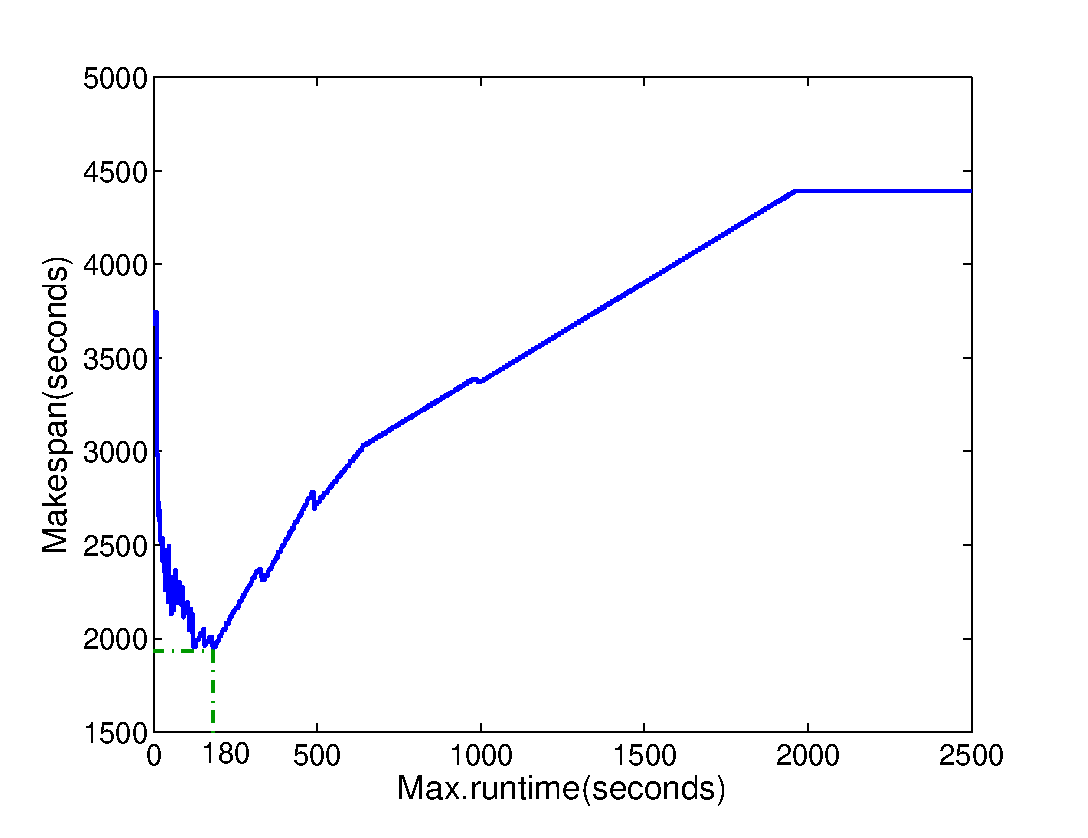
\includegraphics[width=.9\linewidth]{figure19.eps}
	\captionof{figure}{Relationship between the makespan of workflow and the specified maximum runtime in DFJS (Montage).}
	\label{fig:evaluation_dfjs_montage}
\end{figure}

For simplicity, in the rest of this paper we use DFJS* and AFJS* to indicate the best estimated performance of DFJS and AFJS respectively using the sampling approach described above.


% Experiment conditions
\subsection{Experiment conditions}
\label{sec:experiment_conditions}
We adopt a trace-based simulation approach, where we extended our WorkflowSim~\cite{Chen2012a} simulator with the balanced clustering methods and imbalance metrics to simulate a controlled distributed environment. WorkflowSim is a workflow simulator that extends CloudSim~\cite{Calheiros2011} by providing support for task clustering, task scheduling, and resource provisioning at the workflow level. It has been recently used in multiple workflow study areas~\cite{6683907,Chen2012, jrad2013broker} and its correctness has been verified in~\cite{Chen2012a}. 

The simulated computing platform is composed by 20 single homogeneous core virtual machines (worker nodes), which is the quota per user of some typical distributed environments such as Amazon EC2~\cite{AmazonAWS} and FutureGrid~\cite{FutureGrid}. Amazon EC2 is a commercial, public cloud that has been widely used in distributed computing, in particular for scientific workflows~\cite{Juve09scientificworkflow}. FutureGrid is a distributed, high-performance testbed that provides scientists with a set of computing resources to develop parallel, grid, and cloud applications. Each simulated virtual machine (VM) has 512MB of memory and the capacity to process 1,000 million instructions per second. The default network bandwidth is 15MB according to the real environment in FutureGrid from where our traces were collected. The task scheduling algorithm is data-aware, i.e. tasks are scheduled to resources which have the most input data available. By default, we merge tasks at the same horizontal level into 20 clustered jobs, which is a simple selection of granularity control of the strength of task clustering. The study of granularity size has been done in~\cite{6683907}, which shows such selection is acceptable. 

We collected workflow execution traces~\cite{Juve2013,Chen2011} (including overhead and task runtime information) from real runs (executed on FutureGrid and Amazon EC2) of the scientific workflow applications described in Section~\ref{sec:applications}. The traces are used to feed the Workflow Generator toolkit~\cite{FerreiradaSilva-eScience-2014} to generate synthetic workflows. This allows us to perform simulations with several different configurations under controlled conditions. The toolkit uses the information gathered from actual scientific workflow executions to generate synthetic workflows resembling those used by real world scientific applications. The number of inputs to be processed, the number of tasks in the workflow, and their composition determine the structure of the generated workflow. Such an approach of traced based simulation allows us to utilize real traces and vary the system setting (i.e., the number of VMs) and workflow (i.e., avg. data size) to fully explore the performance of our balancing algorithms. 

Three sets of experiments are conducted. Experiment 1 evaluates the performance gain ($\mu$) of our balancing methods (HRB, HIFB, and HDB) over a baseline execution that has no task clustering. We define the performance gain over a baseline execution ($\mu$) as the performance of the balancing methods related to the performance of an execution without clustering. Thus, for values of $\mu > 0$ our balancing methods perform better than the baseline execution. Otherwise, the balancing methods perform poorer. The goal of the experiment is to identify conditions where each method works best and worst. In addition, we also evaluate the performance gain of using workflow structure metrics (HRV, HIFV, and HDV), which require fewer \emph{a-priori} knowledge from task and resource characteristics, over task clustering techniques in literature (HC, DFJS*, and AFJS*).

Experiment 2 evaluates the performance impact of the variation of average data size (defined as the average of all the input and output data) and the number of resources available in our balancing methods for one scientific workflow application (LIGO). The original average data size (both input and output data) of the LIGO workflow is about 5MB as shown in Table~\ref{tab:evaluation_workflows}. In this experiment, we increase the average data size up to 500MB to study the behavior of data intensive workflows. We control resource contention by varying the number of available resources (VMs). High resource contention is achieved by setting the number of available VMs to 5, which represents less than 10\% of the required resources to compute all tasks in parallel. On the other hand, low contention is achieved when the number of available VMs is increased to 25, which represents about 50\% of the required resources.

Experiment 3 evaluates the influence of combining our horizontal clustering methods with vertical clustering (VC). We compare the performance gain under four scenarios: (\emph{i}) \emph{VC-prior}, VC is first performed and then HRB, HIFB, or HDB; (\emph{ii}) \emph{VC-posterior}, horizontal methods are performed first and then VC; (\emph{iii}) \emph{No-VC}, horizontal methods only; and (\emph{iv}) \emph{VC-only}, no horizontal methods. Table~\ref{tab:evaluation_vc_combination} shows the results of combining VC with horizontal methods. For example, VC-HIFB indicates we perform VC first and then HIFB. 
%The motivation behind this experiment is that we believe VC will change imbalance metrics (HIFV, HDV and HRV) and we aim to show how these metrics can help us understand the performance of VC better. 

\begin{table}[!htb]
	%\setlength{\tabcolsep}{11pt}
	\centering
	\small
	\begin{tabular}{l|rrrr}
		\hline
		Combination	& HIFB	 &  HDB & HRB & HC \\
		\hline
		VC-prior 		& VC-HIFB		& VC-HDB	& VC-HRB & VC-HC\\
		VC-posterior 		&HIFB-VC		&HDB-VC	&HRB-VC & HC-VC\\
		VC-only 	&VC		&VC 	& VC & VC\\
		No-VC 	&HIFB 	& HDB & HRB	& HC \\
		\hline
	\end{tabular}
	\caption{Combination Results. `-' indidates the order of performing these algorithms, i.e., VC-HIFB indicates we perform VC first and then HIFB}
	\label{tab:evaluation_vc_combination}
\end{table} 



%With these traces based information, we use WorkflowSim to vary algorithms used, resources, workflow size etc. to illustrate the different runtime performance of these methods. 
%Runtime (average and task runtime distribution) and overhead (workflow engine delay, queue delay, and network bandwidth) information were collected from real traces production environments~\cite{Chen2011, Juve2013}, then used as input parameters for the simulations. 
%where we could evaluate the performance of our methods when varying the average data size and task runtime.


% Results and discussion
\subsection{Results and discussion}
\label{sec:results}
\paragraph{\textbf{Experiment 1}}
Figure~\ref{fig:evaluation_algorithm} shows the performance gain $\mu$ of the balancing methods for the five workflow applications over a baseline execution. All clustering techniques significantly improve (up to 48\%) the runtime performance of all workflow applications, except HC for SIPHT. The reason is that SIPHT has a high HRV compared to other workflows as shown in Table~\ref{tab:evaluation_montage}. This indicates that the runtime imbalance problem in SIPHT is more significant and thus it is harder for HC to achieve performance improvement. Cybershake and Montage workflows have the highest gain but nearly the same performance independent of the algorithm. This is due to their symmetric structure and low values for the imbalance metrics and the distance metrics as shown in Table~\ref{tab:evaluation_montage}. 
Epigenomics and LIGO have higher average task runtime and thus the lower performance gain. However, Epigenomices and LIGO have higher variance of runtime and distance and thus the performance improvement of HRB and HDB is better than that of HC, which is more significant compared to other workflows. 
In particular, each branch of the Epigenomics workflow (Figure~\ref{fig:evaluation_shape_genome}) has the same number of pipelines, consequently the $IF$ values of tasks in the same horizontal level are the same. Therefore, HIFB cannot distinguish tasks from different branches, which leads the system to a dependency imbalance problem. In such cases, HDB captures the dependency between tasks and yields better performance. Furthermore, Epigenomics and LIGO workflows have high runtime variance, which has higher impact on the performance than data dependency. Last, the performance gain of our balancing methods is better than the tuned algorithms DFJS* and AFJS* in most cases. The other benefit is that our balancing methods do not require parameter tuning, which is cumbersome in practice. 

\begin{figure}[htb]
	\centering
	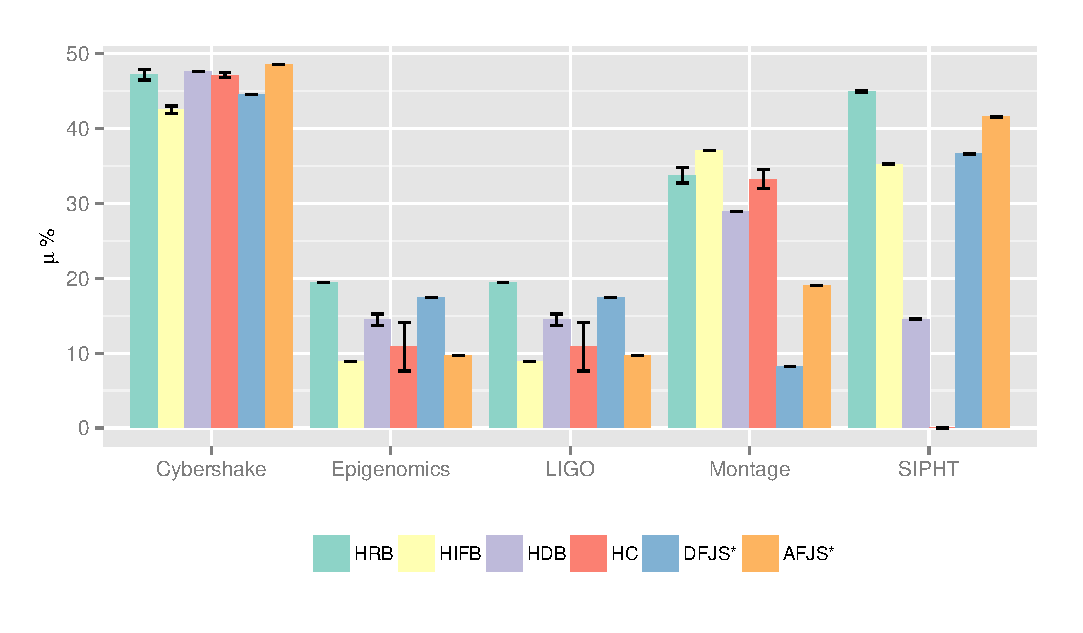
\includegraphics[width=1.0\linewidth]{figure20.eps}
	\captionof{figure}{Experiment 1: performance gain ($\mu$) over a baseline execution for six algorithms (*~indicates the tuned performance of DFJS and AFJS). By default, we have 20 VMs. }
	\label{fig:evaluation_algorithm}
\end{figure}

\begin{table}[!htb]
	\setlength{\tabcolsep}{12pt}
	\centering
	\small
	\begin{tabular}{c|r|r|r|r}
		& \# of Tasks & HRV &  HIFV & HDV  \\ \hline
		Level & \multicolumn{4}{c}{(a) \textbf{CyberShake}} \\
		\hline
		1 & 4 & 0.309 & 0.03 & 1.22 \\
		2 & 347 & 0.282 & 0.00 & 0.00 \\
		3 & 348 & 0.397 & 0.00 & 26.20 \\
		4 & 1 & 0.000 & 0.00 & 0.00 \\
		\hline
		Level & \multicolumn{4}{c}{(b) \textbf{Epigenomics}} \\
		\hline
		1 & 3 & 0.327 & 0.00 & 0.00  \\
		2 & 39 & 0.393 & 0.00 & 578 \\
		3 & 39 & 0.328 & 0.00 & 421 \\
		4 & 39 & 0.358 & 0.00 & 264 \\
		5 &39 & 0.290 & 0.00 & 107 \\
		6 & 3 & 0.247 & 0.00 & 0.00  \\
		7 &1  & 0.000 & 0.00 & 0.00 \\
		8 &1 & 0.000 & 0.00 & 0.00 \\
		9 & 1 & 0.000 & 0.00 & 0.00 \\
		\hline
		Level & \multicolumn{4}{c}{(c) \textbf{LIGO}} \\
		\hline
		1 & 191 & 0.024 & 0.01 & 10097 \\
		2 & 191 & 0.279 & 0.01 & 8264 \\
		3 & 18 & 0.054 & 0.00 & 174 \\
		4 & 191 & 0.066 & 0.01 & 5138 \\
		5 & 191 & 0.271 & 0.01 & 3306 \\
		6 & 18 &  0.040 & 0.00 & 43.70 \\
		\hline		
		Level & \multicolumn{4}{c}{(d) \textbf{Montage}} \\
		\hline
		1 &49 & 0.022 & 0.01 & 189.17 \\
		2 & 196 & 0.010 & 0.00 & 0.00 \\
		3 & 1 & 0.000 & 0.00 & 0.00 \\
		4 & 1 & 0.000 & 0.00 & 0.00 \\
		5 &49 & 0.017 & 0.00 & 0.00 \\
		6 & 1 & 0.000 & 0.00 & 0.00 \\
		7 &1  & 0.000 & 0.00 & 0.00 \\
		8 &1 & 0.000 & 0.00 & 0.00 \\
		9 & 1 & 0.000 & 0.00 & 0.00 \\
		\hline		
		Level & \multicolumn{4}{c}{(e) \textbf{SIPHT}} \\
		\hline
		1 & 712 & 3.356 & 0.01 & 53199 \\
		2 & 64 & 1.078 & 0.01 & 1196 \\
		3 & 128 & 1.719 & 0.00 & 3013 \\
		4 & 32 & 0.000 & 0.00 & 342 \\
		5 & 32 & 0.210 & 0.00 & 228\\
		6& 32 & 0.000 & 0.00 & 114\\
	\end{tabular}
	\caption{Experiment 1: average number of tasks, and average values of imbalance metrics (HRV, HIFV, and HDV) for the 5 workflow applications (before task clustering).}
	\label{tab:evaluation_montage}
\end{table} 


\paragraph{\textbf{Experiment 2}} 
Figure~\ref{fig:evaluation_datasize} shows the performance gain $\mu$ of HRB, HIFB, HDB, and HC over a baseline execution for the LIGO Inspiral workflow. We chose LIGO because the performance improvement among these balancing methods is significantly different for LIGO compared to other workflows as shown in Figure~\ref{fig:evaluation_algorithm}. For small data sizes (up to 100 MB), the application is CPU-intensive and runtime variations have higher impact on the performance of the application. Thus, HRB performs better than any other balancing method. When increasing the data average size, the application turns into a data-intensive application, i.e. data dependencies have higher impact on the application's performance. HIFB captures both the workflow structure and task runtime information, which reduces data transfers between tasks and consequently yields better performance gain over the baseline execution. HDB captures the strong connections between tasks (data dependencies), while HIFB captures the weak connections (similarity in terms of structure). In some cases, HIFV is zero while HDV is less likely to be zero.
Most of the LIGO branches are like the ones in Figure~\ref{fig:evaluation_shape_ligo}, however, as mentioned in Section~\ref{sec:methods}, the LIGO workflow has a few branches that depend on each other as shown in Figure~\ref{fig:imbalance_hifb_hdb}. Since most branches are isolated from each other, HDB initially performs well compared to HIFB. However, with the increase of average data size, the performance of HDB is more and more constrained by the interdependent branches, which is shown in Figure~\ref{fig:evaluation_datasize}.  
HC has nearly constant performance despite of the average data size, due to its random merging of tasks at the same horizontal level regardless of the runtime and data dependency information.

\begin{figure}[!htb]
	\centering
    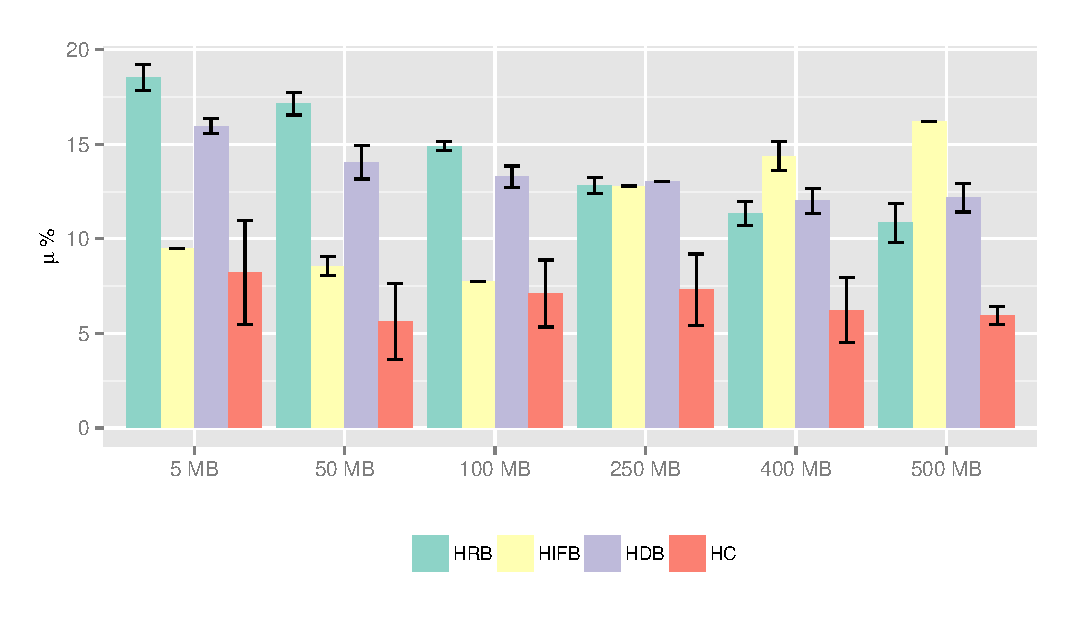
\includegraphics[width=\linewidth]{figure21.eps}
    \caption{Experiment 2: performance gain ($\mu$) over a baseline execution with different average data sizes for the LIGO workflow. The original avg. data size is 5MB.}
    \label{fig:evaluation_datasize}
\end{figure}

Figures~\ref{fig:evaluation_resource_1} and~\ref{fig:evaluation_resource_2} show the performance gain $\mu$ when varying the number of available VMs for the LIGO workflows with an average data size of 5MB (CPU-intensive) and 500MB (data-intensive) respectively. In high contention scenarios (small number of available VMs), all methods perform similar when the application is CPU-intensive (Figure~\ref{fig:evaluation_resource_1}), i.e., runtime variance and data dependency have smaller impact than the system overhead (e.g. queuing time). As the number of available resources increases, and the data size is too small, runtime variance has more impact on the application's performance, thus HRB performs better than the others. Note that as HDB captures strong connections between tasks, it is less sensitive to the runtime variations than HIFB, thus it yields better performance. For the data-intensive case (Figure~\ref{fig:evaluation_resource_2}), data dependencies have more impact on the performance than the runtime variation. In particular, in the high contention scenario HDB performs poor clustering leading the system to data locality problems compared to HIFB due to the interdependent branches in the LIGO workflow. However, the method still improves the execution due to the high system overhead. Similarly to the CPU-intensive case, under low contention, runtime variance increases its importance and then HRB performs better.

\begin{figure}[!htb]
	\centering
	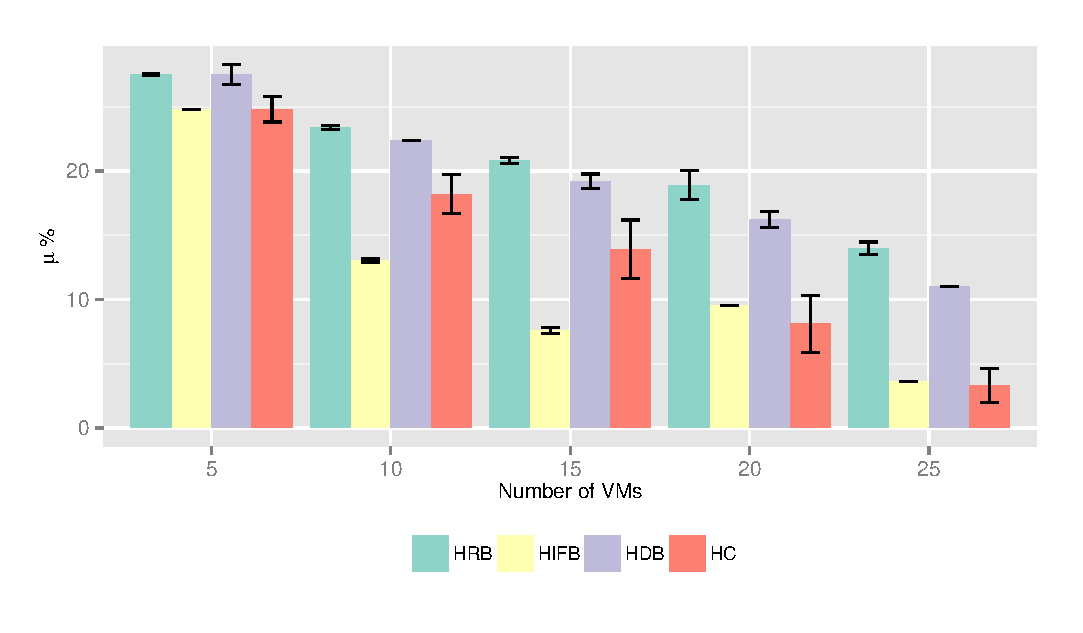
\includegraphics[width=1.0\linewidth]{figure22.eps}
	\captionof{figure}{Experiment 2: performance gain ($\mu$) over baseline execution with different number of resources for the LIGO workflow (average data size is 5MB).}
	\label{fig:evaluation_resource_1}
\end{figure}

\begin{figure}[!htb]
	\centering
	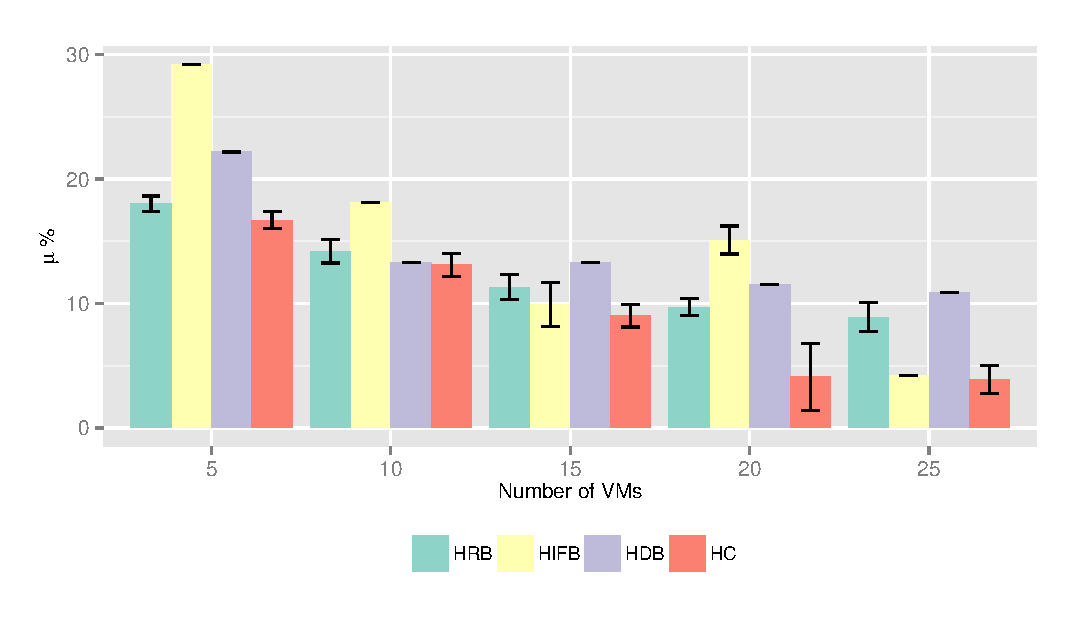
\includegraphics[width=1.0\linewidth]{figure23.eps}
	\captionof{figure}{Experiment 2: performance gain ($\mu$) over baseline execution with different number of resources for the LIGO workflow (average data size is 500MB).}
	\label{fig:evaluation_resource_2}
\end{figure}

To evaluate the performance of our algorithms in a larger scale scenario, we increase the number of tasks in LIGO to 8,000 (following the same structure rules enforced by the WorkflowGenerator toolkit) and simulate the execution with $[200,1800]$ VMs. We choose 1,800 as the maximum number of VMs because the LIGO workflow has a maximum width of 1892 tasks (at the same level). 
%There is little need to perform task clustering if we have more VMs than the width of the workflow.
Figure~\ref{fig:evaluation_resource_3} shows the performance gain over baseline execution with different number of resources for the LIGO workflow. In a small scale (i.e., 200 VMs), HRB and HDB perform slightly better than the other methods. However, as the scale increases, HDB outperforms the other methods. Similarly to the results obtained in Figure~\ref{fig:evaluation_resource_2}, HRB performs worse in larger scales since the runtime imbalance is no longer a major issue (HRV is too small) and thus the dependency imbalance becomes the bottleneck. Within the two dependency-oriented optimization methods, HDB outperforms HIFB since HDB captures the strong relation between tasks (distance), while HIFB uses the impact factor based metrics to capture the structural similarity. 

\begin{figure}[!htb]
	\centering
	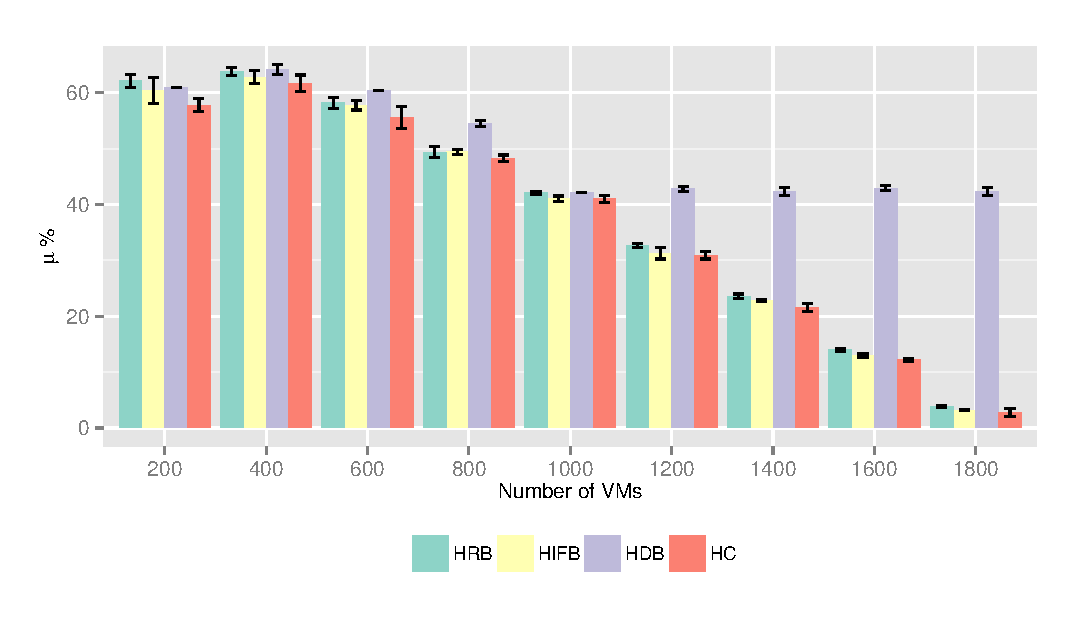
\includegraphics[width=1.0\linewidth]{figure28.eps}
	\captionof{figure}{Experiment 2: performance gain ($\mu$) over baseline execution with different number of resources for the LIGO workflow (number of tasks is 8000).}
	\label{fig:evaluation_resource_3}
\end{figure}

\paragraph{\textbf{Experiment 3}}
Figure~\ref{fig:evaluation_vc_cybershake} shows the performance gain $\mu$ for the Cybershake workflow over the baseline execution when using vertical clustering (VC) combined to our balancing methods. Vertical clustering does not aggregate any improvement to the Cybershake workflow ($\mu$(\emph{VC-only}) $\approx 0.2\%$), because the workflow structure has no explicit pipeline (see Figure~\ref{fig:evaluation_shape_cybershake}). Similarly, VC does not improve the SIPHT workflow due to the lack of pipelines on its structure (Figure~\ref{fig:evaluation_shape_sipht}). Thus, results for this workflow are omitted.

\begin{figure}[!htb]
	\centering
	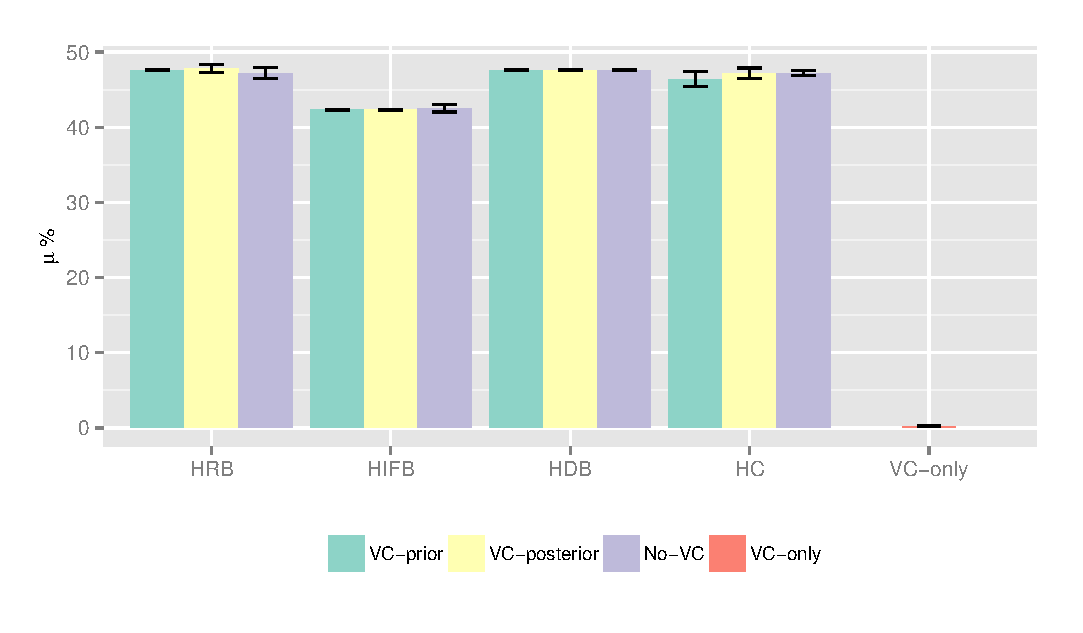
\includegraphics[width=1.0\linewidth]{figure24.eps}
	\captionof{figure}{Experiment 3: performance gain ($\mu$) for the Cybershake workflow over baseline execution when using vertical clustering (VC).}
	\label{fig:evaluation_vc_cybershake}
\end{figure}

Figure~\ref{fig:evaluation_vc_montage} shows the performance gain $\mu$ for the Montage workflow. In this workflow, vertical clustering is often performed on the two pipelines (Figure~\ref{fig:evaluation_shape_montage}). These pipelines are commonly single-task levels, thereby no horizontal clustering is performed on the pipelines. As a result, whether performing vertical clustering prior or after horizontal clustering, the result is about the same. Since VC and horizontal clustering methods are independent with each other in this case, we still should do VC in combination with horizontal clustering to achieve further performance improvement. 

\begin{figure}[!htb]
	\centering
	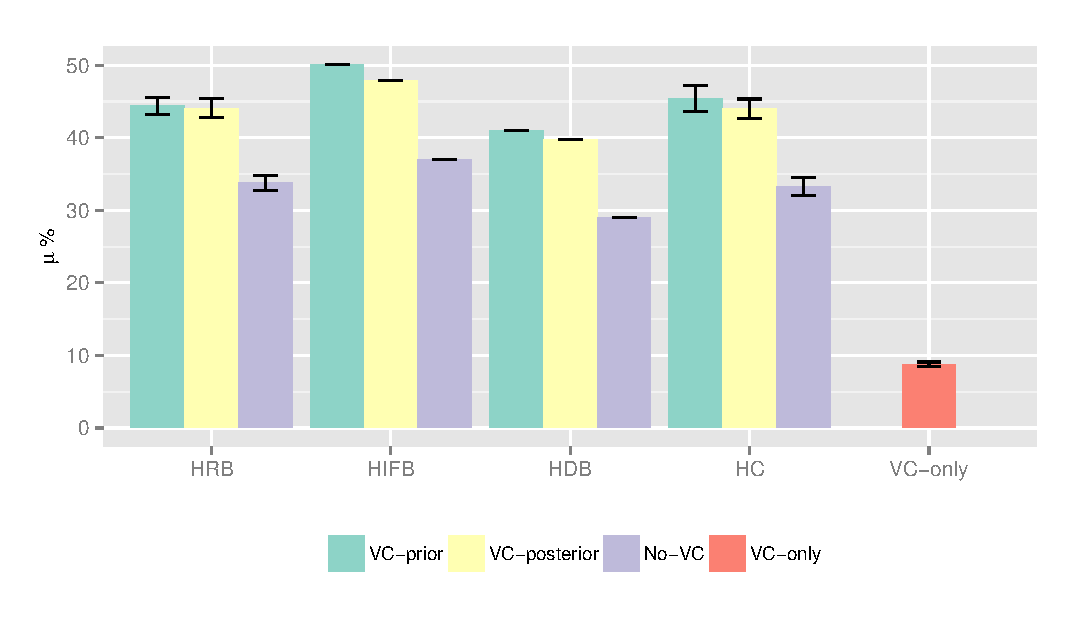
\includegraphics[width=1.0\linewidth]{figure25.eps}
	\captionof{figure}{Experiment 3: performance gain ($\mu$) for the Montage workflow over baseline execution when using vertical clustering (VC).}
	\label{fig:evaluation_vc_montage}
\end{figure}

\begin{figure}[!htb]
	\centering
	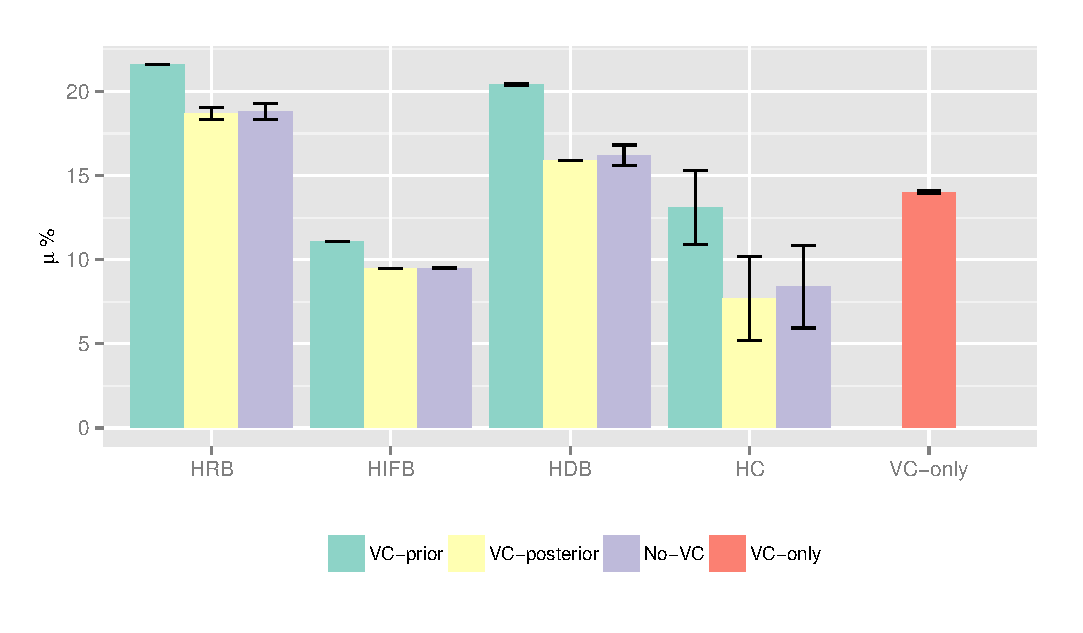
\includegraphics[width=1.0\linewidth]{figure26.eps}
	\captionof{figure}{Experiment 3: performance gain ($\mu$) for the LIGO workflow over baseline execution when using vertical clustering (VC).}
	\label{fig:evaluation_vc_ligo}
\end{figure}


\begin{figure}[!htb]
	\centering
	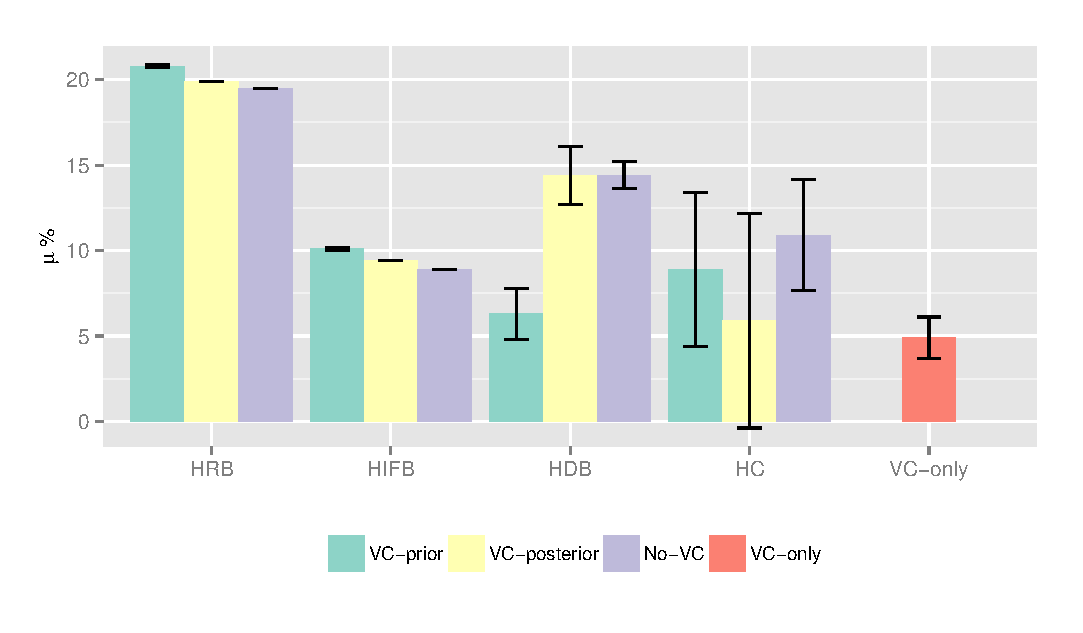
\includegraphics[width=1.0\linewidth]{figure27.eps}
	\captionof{figure}{Experiment 3: performance gain ($\mu$) for the Epigenomics workflow over baseline execution when using vertical clustering (VC).}
	\label{fig:evaluation_vc_genome}
\end{figure}

The performance gain $\mu$ for the LIGO workflow is shown in Figure~\ref{fig:evaluation_vc_ligo}. Vertical clustering yields better performance gain when it is performed prior to horizontal clustering (\emph{VC-prior}). The LIGO workflow structure (Figure~\ref{fig:evaluation_shape_ligo}) has several pipelines that are primarily clustered vertically and thus system overheads (e.g. queuing and scheduling times) are reduced. Furthermore, the runtime variance (HRV) of the clustered pipelines increases, thus the balancing methods, in particular HRB, can further improve the runtime performance by evenly distributing task runtimes among clustered jobs. When vertical clustering is performed \emph{a posteriori}, pipelines are broken due to the horizontally merging of tasks between pipelines neutralizing vertical clustering improvements.

Similarly to the LIGO workflow, the performance gain $\mu$ values for the Epigenomics workflow (see Figure~\ref{fig:evaluation_vc_genome}) are better when VC is performed \emph{a priori}. This is due to several pipelines inherent to the workflow structure (Figure~\ref{fig:evaluation_shape_genome}). However, vertical clustering has poorer performance if it is performed prior to the HDB algorithm. The reason is the average task runtime of Epigenomics is much larger than other workflows as shown in Table.~\ref{tab:evaluation_workflows}. Therefore, \emph{VC-prior} generates very large clustered jobs vertically and makes it difficult for horizontal methods to improve further. 


\subsection{Compilation of the results}

The experimental results show strong relations between the proposed imbalance metrics and the performance improvement of the balancing methods. HRV indicates the potential performance improvement for HRB. The higher HRV, the more performance improvement HRB is likely to have. Similarly, for workflows with symmetric structures (such as Epigenomics) where HIFV and HDV values are low, neither HIFB nor HDB performs well.

Based on the conclusions of the experimental evaluation, we applied machine learning techniques on the result data to build a decision tree that can be used to drive the development of police engines to interactively select a balancing method. Although our decision tree is tightly coupled to our results, it can be used by online systems that implement the MAPE-K loop~\cite{daSilva:2013:TFO:2534248.2534254,FerreiradaSilva-CCPE-2014,FerreiradaSilva-FGCS-2013}, which will adjust the tree according to the system behavior.

\begin{figure}[!htb]
	\centering
	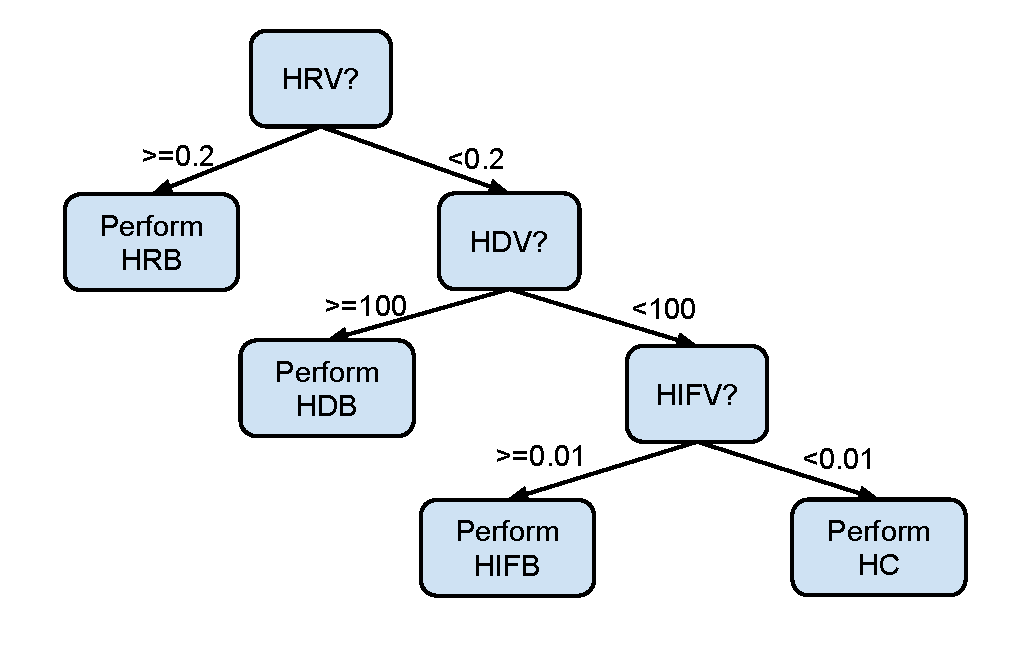
\includegraphics[width=1.0\linewidth]{tree.pdf}
	\captionof{figure}{Decision tree for selection of the appropriate balancing method.}
	\label{fig:decision_tree}
\end{figure}



%For the Epigenomics workflow as shown in Figure~\ref{fig:evaluation_vc_genome}, we observe similar phenomenon in HRB compared to the LIGO Inspiral workflow. As to the performance of HDB, VC-prior merges tasks at the second, third, fourth and fifth level together and thus HDB has less space to further improve the overall runtime. 

%Figure~\ref{fig:evaluation_wfsize} compares the performance gain of these algorithms by varying the workflow sizes (number of tasks in a workflow). By default, the LIGO Inspiral workflow in our paper has 800 tasks. With the decrease of workflow size, we can see that all of these methods perform worse. The reason is there is less resource contention with the decrease of workflow size and therefore task clustering does not perform well. The performance of HRB is more stable since the increase (or decrease) of workflow size has more significant impact on data transfer (roughly linear increase in runtime and square increase in data transfer). 

%The SIPHT workflow as shown in Figure~\ref{fig:evaluation_shape_sipht} does not have enough pipelines to perform vertical clustering and therefore we do not show its results of combining vertical clustering. 
 
%HIFB and HDB significantly increase the performance of the workflow execution. Both strategies capture the structural and runtime information, reducing data transfers between tasks, while HRB focuses on runtime distribution, which in this case is none. Figure~\ref{fig:imbalance_performance} (bottom) shows the performance of the balancing methods for the Epigenomics workflow. When increasing the average data size, only HDB demonstrates significantly improvement related to HC. Investigating the structure of the Epigenomics workflow (Figure~\ref{fig:imbalance_shape}-bottom), we can see that all tasks at the same horizontal level share the same IFs ($HIFV$ = 0), because each branch (surrounded by dash lines) happen to have the same amount of pipelines. Thus, HIFB has no performance improvement when compared to HC. However, for LIGO (Figure~\ref{fig:imbalance_shape}-top), $HIFV \neq 0$, thus HIFB improves the workflow runtime performance.  
%The intuition behind this difference between HDB and HIFB is that 
%HDB captures the strong connections between tasks (data dependencies) and HIFB captures the weak connections (similarity in terms of structure). In both workflows, $HDV$ is not zero thus HDB performs better than HC. 






